\chapter{宁国府除夕祭宗祠 \quad 荣国府元宵开夜宴}
\qi{除夕祭宗祠一题极博大,元宵开夜宴一题极富丽,拟此二题于一回中,早令人惊心动魄。
不知措手处,乃作者偏就宝琴眼中款款叙来。
首叙院宇匾对,次叙抱厦匾对,后叙正堂匾对,字字古艳。
槛以外,槛以内,是男女分界处;仪门以外,仪门以内,是主仆分界处。
献帛献爵择其人,\zhu{献帛:祭祀礼仪之一,“帛”指缯帛、币帛,作为供品的一种绣织精美的丝织品。
爵:古代一种酒器。
献爵:犹献酒,敬酒。
}应昭应穆从其讳,\zhu{昭穆:古代宗法制度对于宗庙祭祀排列次序的规定,始祖居中,始祖的下一代为昭,居左,昭辈的下一代为穆,居右;穆辈的下一代又为昭,居左;以后各代,依此类推;用以区别父子、远近、长幼、亲疏等关系。
讳:封建社会称死去的帝王或尊长的名。
这里是指贾府按字排辈,比如贾代化、贾代善是“代”字辈,贾敬、贾赦是“文”字辈(右边的偏旁为“文”),贾珠、贾珍是“玉”字辈(左边偏旁为“玉”),贾蓉、贾芸是“草”字辈(上面偏旁是“草”)。
根据名中的字,就可以知道一个人的辈分和应该归属昭还是穆。
}是一篇绝大典制文字。
最高妙是神主看不真切一句,最苦心是用贾蓉为槛边传蔬人,用贾芷等为仪门传蔬人,体贴入细。
噫!文心至此,脉绝血枯矣。
谁是知音者?}\par
话说宝玉见晴雯将雀裘补完,已使的力尽神危,忙命小丫头子来替他捶着,彼此捶打了一会歇下。
\zhu{彼此:这里不是双向的,而是偏向一方。
}没一顿饭的工夫,天已大亮,且不出门,只叫快传大夫。
一时王太医来了,诊了脉,疑惑说道:“昨日已好了些,今日如何反虚浮微缩起来,\zhu{虚浮微缩:中医诊断脉象的术语。
虚、微:指脉搏细软无力的脉象,常见于正气不足、气血虚极的各种疾病。
浮、缩:指轻按便得、重按反觉减弱的脉象。
病初起,邪在表时,出现浮脉是正常的;病久后,正气损伤,致使气血运行不通畅,正常的情况应出现沉脉(沉脉是指脉象位置较低深,用指轻取不可得,重按方得的脉象);如果相反地出现了浮脉,说明阳气已不能潜藏,病情已到十分危重的地步。
故王太医认为晴雯病已“非同小可”。
}敢是吃多了饮食?不然就是劳了神思。
外感却倒清了,\zhu{外感:指感受风、寒、暑、湿、燥、热而致病。
内滞:在消化系统内有饮食积滞。
}这汗后失于调养,非同小可。
一面说,一面出去开了药方进来。
宝玉看时,已将疏散驱邪诸药减去了,倒添了茯苓、地黄、当归等益神养血之剂。
宝玉忙命人煎去,一面叹说:“这怎么处!倘或有个好歹,都是我的罪孽。
”晴雯睡在枕上嗐道:
\zhu{嗐:音“害”,表示不满,惋惜或懊悔。}
“好太爷!你干你的去罢!那里就得痨病了。
”宝玉无奈,只得去了。
至下半天,说身上不好就回来了。
晴雯此症虽重,幸亏他素习是个使力不使心的;再者素习饮食清淡,饥饱无伤。
这贾宅中的风俗秘法,无论上下,只一略有些伤风咳嗽,总以净饿为主,次则服药调养。
故于前日一病时,净饿了两三日,又谨慎服药调治,如今劳碌了些,又加倍培养了几日,便渐渐的好了。
近日园中姊妹皆各在房中吃饭,炊爨饮食亦便,\zhu{爨:音“篡”,烧火做饭;灶。
}宝玉自能变法要汤要羹调停,
\zhu{调停:照料,安排(多见于早期白话)。}
不必细说。
\par
袭人送母殡后,业已回来,麝月便将平儿所说宋妈坠儿一事,并晴雯撵逐出去等话,一一也曾回过宝玉。
袭人也没别说,只说太性急了些。
只因李纨亦因时气感冒;邢夫人又正害火眼,\zhu{火眼:即急性结膜炎,俗称“红眼病”。
}迎春岫烟皆过去朝夕侍药;\geng{妙在一人不落,事事皆到。
}李婶之弟又接了李婶和李纹李绮家去住几日;\geng{来得也有理,去得也有情。
}宝玉又见袭人常常思母含悲,晴雯犹未大愈:因此诗社之日,皆未有人作兴,\zhu{作兴:举办,使之兴盛。
}便空了几社。
\par
当下已是腊月,离年日近,王夫人与凤姐治办年事。
王子腾升了九省都检点,\zhu{都检点:亦作都点检,官名,五代置,为禁军最高统帅,宋初废。
这里借指朝廷委派的高级武官。
}贾雨村补授了大司马,\zhu{大司马:官名,汉置,掌管内廷全部政务,后世用作兵部尚书的别称。
}协理军机参赞朝政,\zhu{参:参加,参与。
赞:辅助,辅佐。
}不题。
\par
且说贾珍那边,开了宗祠,着人打扫,收拾供器,请神主,又打扫上房,以备悬供遗真影像。
此时荣宁二府内外上下,皆是忙忙碌碌。
这日,宁府中尤氏正起来,同贾蓉之妻打点送贾母这边针线礼物,正值丫头捧了一茶盘押岁锞子进来,\zhu{
押岁:又叫“压岁”。春节拜年时,长辈要将事先准备好的压岁钱分给晚辈。据说,压岁钱可以压住邪祟,因为“岁”与“祟”谐音,晚辈得到压岁钱就可以平平安安度过一年。
主子也有送童仆、丫鬟押岁钱的。
锞子(锞音“课”):旧时做货币用的小金锭或银锭。
}回说:“兴儿回奶奶,前儿那一包碎金子共是一百五十三两六钱七分,里头成色不等,共总倾了二百二十个锞子。
”\zhu{倾:这里指将金银熔化倒入模子里铸造的一种工艺。
古代使用金银作为货币,需将大锭化小,或集零为整,或铸成各种特定的形状(如锞子),都叫作“倾”。
}说着递上去。
尤氏看了看,只见也有梅花式的,也有海棠式的,也有笔锭如意的,\zhu{笔锭如意:有笔和如意为纹饰的金银锞子。以“笔锭”谐音“必定”,意谓一定吉祥、事事如意。
}也有八宝联春的。
\zhu{八宝联春:八宝是八种表示吉庆祥瑞之物。
将这八宝铸在一起,就成为八宝连春。
}尤氏命:“收起这个来,叫他把银锞子快快交了进来。
”丫鬟答应去了。
\par
一时贾珍进来吃饭,贾蓉之妻回避了。
\ping{贾珍和贾蓉的第二个媳妇规矩了……}贾珍因问尤氏:“咱们春祭的恩赏可领了不曾?”\zhu{春祭的恩赏:旧历年节,皇帝按照常例赏给受封荫的官僚供祭祖用的银两。
}尤氏道:“今儿我打发蓉儿关去了。
”\zhu{关:领取。
}贾珍道:“咱们家虽不等这几两银子使,多少是皇上天恩。
早关了来,给那边老太太见过,置了祖宗的供,上领皇上的恩,下则是托祖宗的福。
咱们那怕用一万银子供祖宗,到底不如这个,又体面,又是沾恩锡福的。
\zhu{锡:音“次”,赐。
}除咱们这样一二家之外,那些世袭穷官儿家,若不仗着这银子,拿什么上供过年?真正皇恩浩大,想的周到。
”尤氏道:“正是这话。
”\par
二人正说着,只见人回:“哥儿来了。
”贾珍便命叫他进来。
只见贾蓉捧了一个小黄布口袋进来。
贾珍道:“怎么去了这一日。
”贾蓉陪笑回说:“今儿不在礼部关领,又分在光禄寺库上,\zhu{光禄寺:官署名,自北齐起光禄寺掌管皇室膳食,历朝相沿,至清代,皇帝膳饮由内务府掌管,光禄寺为外廷职司,只管祭祀所用膳食等事。
}因又到了光禄寺才领了下来。
光禄寺的官儿们都说问父亲好,多日不见,都着实想念。
”贾珍笑道:“他们那里是想我。
这又到了年下了,不是想我的东西,就是想我的戏酒了。
”一面说,一面瞧那黄布口袋,上有印就是“皇恩永锡”四个大字,那一边又有礼部祠祭司的印记,又写着一行小字,道是“宁国公贾演、荣国公贾源,恩赐永远春祭赏共二分,净折银若干两,某年月日龙禁尉候补侍卫贾蓉当堂领讫,\zhu{讫:音“气”,终了,完毕。
}值年寺丞某人”,\zhu{值:当差,担任工作,值班。
值年:以一年为周期轮流负责,轮到负责的那一年为值年。
}下面一个朱笔花押。
\zhu{花押:旧时文书契约末尾的草书签名或代替签名的特种符号。
}\par
贾珍吃过饭,盥漱毕,换了靴帽,命贾蓉捧着银子跟了来,回过贾母王夫人,又至这边回过贾赦邢夫人,方回家去,取出银子,命将口袋向宗祠大炉内焚了。
又命贾蓉道:“你去问问你琏二婶子,正月里请吃年酒的日子拟了没有。
若拟定了,叫书房里明白开了单子来,咱们再请时,就不能重犯了。
旧年不留心重了几家,不说咱们不留神,倒像两宅商议定了送虚情怕费事一样。
”贾蓉忙答应了过去。
一时,拿了请人吃年酒的日期单子来了。
贾珍看了,命交与赖升去看了,请人别重这上头日子。
因在厅上看着小厮们抬围屏,擦抹几案金银供器。
只见小厮手里拿着个禀帖并一篇帐目,回说:“黑山村的乌庄头来了。
”\zhu{庄头:清代为满汉旗籍贵族地主经营旗地田庄的代理人,专管监督佃户生产,催收地租,摊派劳役等事,有的庄头本身就是地主。
}\par
贾珍道:“这个老砍头的今儿才来。
”说着,贾蓉接过禀帖和帐目,忙展开捧着,贾珍倒背着两手,向贾蓉手内看红禀帖上写着\foot{原作“向贾蓉手内只看红禀帖上写着”,似有错夺,故各本有所校改:“只看”蒙本作“看那”,甲辰、杨本作“看去那”,也未见佳;列本此处有删削;现依戚本酌删“只”字。
}:“门下庄头乌进孝叩请爷、奶奶万福金安,并公子小姐金安。
新春大喜大福,荣贵平安,加官进禄,万事如意。
”
\ping{
乌进孝,乌表示疑问或反问,相当于“哪里”、“怎么”。
乌进孝可能是暗指没有进孝。
况且年纪大了还要亲历亲为送货,可能正是因为有克扣不足,觉得自己儿子对付不了东家。
庄头相当于包税人,有的庄头本身也是地主。
自耕农(佃农)、地主、政府(皇帝亲贵)三者有复杂的矛盾关系。
自耕农(佃农)是劳动产品的生产者,地主和政府(皇帝亲贵)都是劳动产品的消费者,这是一层剥削与被剥削的矛盾。
在剥削阶级内部,皇帝不直接管理农民,而是委托地主管理,皇帝和地主对于剥削收益的分配也有矛盾。
地主有动机隐瞒人口和收入,少向皇帝交税。
}
贾珍笑道:“庄家人有些意思。
”贾蓉也忙笑说:“别看文法,只取个吉利罢了。
”一面忙展开单子看时,只见上面写着:“大鹿三十只,\ping{鹿通禄,禄的意思是福气,也指官吏的薪俸。
}獐子五十只,狍子五十只,
\zhu{狍[páo]子:鹿科草食动物。}
暹猪二十个,\zhu{
暹猪:暹罗进贡的猪。
暹罗:音“先罗”,泰国的旧称。
}
汤猪二十个,\zhu{汤:汤即“烫”,汤猪即为烫猪,即可烫去毛连皮食用的猪。
食猪,将猪杀死后,习惯把猪皮全部剥下来。
汤猪是杀后不剥皮,只用热开水将毛褪下,连皮食用的,一般用嫩皮小猪。
汤羊类似。
}龙猪二十个,\zhu{龙猪:一种长毛猪种,多瘦肉,少肥肉。}野猪二十个,家腊猪二十个,野羊二十个,青羊二十个,家汤羊二十个,家风羊二十个,\zhu{风羊:将羊杀死后,不煺毛,不剥皮,只把五脏取出,将五香盐料放进肚里,风干,叫做“风羊”。
}鲟鳇鱼二十个,各色杂鱼二百斤,活鸡、鸭、鹅各二百只,风鸡、鸭、鹅二百只,\zhu{风鸡:腌制风干的鸡。
鸡杀后不去毛,除去内脏,在腹内抹上花椒、盐等,风干而成。
风鸭、风鹅类似。
}野鸡、兔子各二百对,熊掌二十对,鹿筋二十斤,海参五十斤,鹿舌五十条,牛舌五十条,蛏干二十斤,
\zhu{蛏[chēnɡ]:软体动物,有两扇介壳,形状狭而长。}
榛、松、桃、杏穰各二口袋,
\zhu{穰:同“瓤”。}
大对虾五十对,干虾二百斤,银霜炭上等选用一千斤、中等二千斤,\zhu{银霜炭:一种优质无烟炭,表面灰白,如披银霜。
}柴炭三万斤,御田胭脂米二石,\zhu{御田胭脂米:一种优质稻米,煮熟后色红如胭脂,有香气,味腴粒长。
据清代刘廷玑《在园杂志》及《顺天府志》记载,胭脂米是康熙帝在丰泽园御田布种的玉田稻中的良种,因而也叫“玉田米”,为内膳所用。
七十五回贾母所吃的“红稻米粥”亦当指此。
石[dàn]:容量单位,十斗为一石。
重量单位,一百二十斤为一石。
}\geng{《在园杂\sout{字}[志]》曾有此说。
}碧糯五十斛,\zhu{糯[nuò]:黏性的稻米。斛:音“胡”,古量器名,也是容量单位,十斗为一斛,南宋末年改五斗为一斛。
}白糯五十斛,粉粳五十斛,
\zhu{粳[jīng]:稻之不黏者。}
杂色粱谷各五十斛,下用常米一千石,各色干菜一车,外卖粱谷、牲口各项之银共折银二千五百两。
外门下孝敬哥儿姐儿顽意:活鹿两对,活白兔四对,黑兔四对,活锦鸡两对,西洋鸭两对。
”\par
贾珍便命带进他来。
一时,只见乌进孝进来,只在院内磕头请安。
贾珍命人拉他起来,笑说:“你还硬朗。
”乌进孝笑回:“托爷的福,还能走得动。
”贾珍道:“你儿子也大了,该叫他走走也罢了。
”乌进孝笑道:“不瞒爷说,小的们走惯了,不来也闷的慌。
他们可不是都愿意来见见天子脚下世面?他们到底年轻,怕路上有闪失,再过几年就可放心了。
”贾珍道:“你走了几日?”乌进孝道:“回爷的话,今年雪大,外头都是四五尺深的雪,前日忽然一暖一化,路上竟难走的很,耽搁了几日。
虽走了一个月零两日,因日子有限了,怕爷心焦,可不赶着来了。
”贾珍道:“我说呢,怎么今儿才来。
我才看那单子上,今年你这老货又来打擂台来了。
”\zhu{打擂台:设台比武,引申为耍花招、较量手段、存心作对。
}乌进孝忙进前了两步,回道:“回爷说,今年年成实在不好。
从三月下雨起,接接连连直到八月,竟没有一连晴过五日。
九月里一场碗大的雹子,方近一千三百里地,连人带房并牲口粮食,打伤了上千上万的,所以才这样。
小的并不敢说谎。
”贾珍皱眉道:“我算定了你至少也有五千两银子来,这够作什么的!如今你们一共只剩了八九个庄子,今年倒有两处报了旱涝,你们又打擂台,真真是又教别过年了。
”乌进孝道:“爷的这地方还算好呢!我兄弟离我那里只一百多里,谁知竟大差了。
他现管着那府里八处庄地,比爷这边多着几倍,今年也只这些东西,不过多二三千两银子,也是有饥荒打呢。
”\zhu{饥荒:犹亏空。
}贾珍道:“正是呢,我这边都可以,没有什么外项大事,不过是一年的费用。
费些我就受用些,我受些委屈就省些。
再者年例送人请人,我把脸皮厚些,可省些也就完了。
比不得那府里,这几年添了许多花钱的事,一定不可免是要花的,却又不添些银子产业。
这一二年倒赔了许多,不和你们要,找谁去!”乌进孝笑道:“那府里如今虽添了事,有去有来,娘娘和万岁爷岂不赏的!”\geng{是庄头口中语气。
脂砚。
}贾珍听了,笑向贾蓉等道:“你们听,他这话可笑不可笑?”贾蓉等忙笑道:“你们山坳海沿子上的人,那里知道这道理。
娘娘难道把皇上的库给了我们不成!他心里纵有这心,他也不能作主。
岂有不赏之理,按时到节不过是些彩缎古董顽意儿。
纵赏银子,不过一百两金子,才值了一千两银子,够一年的什么?这二年那一年不多赔出几千银子来!头一年省亲连盖花园子,你算算那一注共花了多少,就知道了。
再两年再一回省亲,只怕就净穷了。
”贾珍笑道:“所以他们庄家老实人,外明不知里暗的事。
黄柏木作磬槌子——外头体面里头苦。
”\geng{新鲜趣语。
}\zhu{
黄柏,一种落叶乔木,味苦。
槌[chuí]:类似棒子的敲打用具,一般一头较粗或为球形。
黄柏木作磬槌子——外头体面里头苦:
比喻外表看起来很光采,可是内里有很多难言之隐。
}贾蓉又笑向贾珍道:“果真那府里穷了。
前儿我听见凤姑娘\geng{此亦南北互用之文,前注不谬。
\zhu{第五十二回批语:此“姑娘”亦“姑姑”“娘娘”之称,亦如贾琏处小厮呼平儿,皆南北互用一语也。
脂砚。
这里的“姑娘”的意思是“姑姑”。
}}和鸳鸯悄悄商议,要偷出老太太的东西去当银子呢。
”\ping{第七十二回,贾琏求鸳鸯偷出来贾母的东西,典当银子填补财务亏空。
}贾珍笑道:“那又是你凤姑娘的鬼,那里就穷到如此。
他必定是见去路太多了,实在赔的狠了,不知又要省那一项的钱,先设此法使人知道,说穷到如此了。
我心里却有一个算盘,还不至如此田地。
”说着,命人带了乌进孝出去,好生待他,不在话下。
\par
这里贾珍吩咐将方才各物,留出供祖的来,将各样取了些,命贾蓉送过荣府里。
然后自己留了家中所用的,馀者派出等例来,一分一分的堆在月台下,命人将族中的子侄唤来与他们。
接着荣国府也送了许多供祖之物及与贾珍之物。
贾珍看着收拾完备供器,靸着鞋,\zhu{靸:音“洒”,穿鞋时把鞋后帮踩在脚后跟下,拖着走。
}披着猞猁狲大裘,\zhu{猞猁狲:音“奢力孙”,兽名,猞猁的别称,亦名土豹。
毛呈红色或灰色,常带黑斑。
其皮毛可作衣裘,很贵重。
}命人在厅柱下石矶上太阳中铺了一个大狼皮褥子,负暄闲看各子弟们来领取年物。
\zhu{负暄:即“负日之暄”,晒太阳取暖的意思。
暄,音“宣”,暖和。
}因见贾芹亦来领物,贾珍叫他过来,说道:“你作什么也来了?谁叫你来的?”贾芹垂手回说:“听见大爷这里叫我们领东西,我没等人去就来了。
”贾珍道:“我这东西,原是给你那些闲着无事的无进益的小叔叔兄弟们的。
那二年你闲着,我也给过你的。
你如今在那府里管事,家庙里管和尚道士们,一月又有你的分例外,这些和尚的分例银子都从你手里过,你还来取这个,太也贪了!你自己瞧瞧,你穿的像个手里使钱办事的?先前说你没进益,如今又怎么了?比先倒不像了。
”贾芹道:“我家里原人口多,费用大。
”贾珍冷笑道:“你还支吾我。
你在家庙里干的事,打量我不知道呢。
你到了那里自然是爷了,没人敢违拗你。
你手里又有了钱,离着我们又远,你就为王称霸起来,夜夜招聚匪类赌钱,\geng{这一回文字断不可少。
}养老婆小子。
\zhu{老婆、小子:分别指女性和男性性伙伴。}
这会子花的这个形象,你还敢领东西来?领不成东西,领一顿驮水棍去才罢。
\zhu{驮水棍:背水负重时用作支撑的随身棍棒。
这里借指打人棍棒。
“领一顿驮水棍”即“招一顿打”的意思。
}等过了年,我必和你琏二叔说,换回你来。
”贾芹红了脸,不敢答应。
人回:“北府水王爷送了字联、荷包来了。
”贾珍听说,忙命贾蓉出去款待,“只说我不在家。
”\ping{贾珍作为贾家族长,为何在这里如此害羞呢?}贾蓉去了,这里贾珍看着领完东西,回房与尤氏吃毕晚饭,一宿无话。
至次日,更比往日忙,都不必细说。
\par
已到了腊月二十九日了,各色齐备,两府中都换了门神、联对、挂牌,新油了桃符,\zhu{桃符:称画有门神像或题有门神名的桃木板为桃符,又春联也称桃符。
}焕然一新。
宁国府从大门、仪门、大厅、暖阁、内厅、内三门、内仪门并内塞门,\zhu{内塞门:塞门即屏门,设屏于门,以蔽内外也。
这里的内塞门,即内仪门与正堂间的又一重屏门。
}直到正堂,一路正门大开,两边阶下一色朱红大高照,点的两条金龙一般。
次日,由贾母有诰封者,\zhu{诰封:音“告封”,明清对五品以上官员及其先代和妻室以皇帝的诰命授予封典,谓“诰封”。
}皆按品级着朝服,先坐八人大轿,带领着众人进宫朝贺,行礼领宴毕回来,便到宁国府暖阁下轿。
诸子弟有未随入朝者,皆在宁府门前排班伺候,然后引入宗祠。
且说宝琴是初次,一面细细留神打量这宗祠,原来宁府西边另一个院子,黑油栅栏内五间大门,
\zhu{
五间大门:乾隆二十九年(1764)钦定的《大清会典》规定:“凡亲王府制,正门五间,启门三。”
明确规定亲王府,包括郡王府,可以构筑五间大门,但是只能开启中间的三间大门,也就“五启三”。
}
上悬一块匾,写着是“贾氏宗祠”四个字,旁书“衍圣公孔继宗书”。
\zhu{衍圣公:孔子后裔的封号,自宋仁宗时始,历朝沿袭。
}两旁有一副长联,写道是:\par
\hop
肝脑涂地,兆姓赖保育之恩;\par
功名贯天,百代仰蒸尝之盛。
\zhu{蒸尝:古代祭祀名。
《尔雅·释天》:“秋祭曰尝,冬祭曰蒸。
”} \par
\hop
亦衍圣公所书。
进入院中,白石甬路,两边皆是苍松翠柏。
月台上设着青绿古铜鼎彝等器。
\zhu{
月台:正殿或正房前面凸出的平台。
彝:音“遗”,古代青铜器的通称,多指宗庙祭祀用的礼器。
}抱厦前上面悬一九龙金匾,写道是:“星辉辅弼”。
\zhu{星辉辅弼:代指辅佐帝王的重臣。
以日月比帝王,以星辰比大臣。
弼,音“币”,辅佐。
}
乃先皇御笔。
两边一副对联,写道是:\par
\hop
勋业有光昭日月,功名无间及儿孙。
\zhu{间:音“见”,空间或时间上的间断。
}\par
\hop
亦是御笔。
五间正殿前悬一闹龙填青匾,\zhu{闹龙填青匾:匾的四边雕镂以舞动的龙形图案,谓之“闹龙”;匾的底面作石青色,谓之“填青”。
}写道是:“慎终追远”。
\zhu{慎终追远:语出《论语·学而》。
慎终:父母亡故做到居丧尽礼;追远:按时诚敬地祭祀祖先。
这里引申为谨慎从事,考虑身后,追念先人,保持祖德。
}旁边一副对联,写道是:\par
\hop
已后儿孙承福德,至今黎庶念荣宁。
\par
\hop
俱是御笔。
里边香烛辉煌,锦帐绣幕,虽列着神主,却看不真切。
\ping{从宝琴眼中写来,因为离得远,所以看不真切。
}只见贾府人分昭穆排班立定:\zhu{昭穆:古代宗法制度对于宗庙祭祀排列次序的规定,始祖居中,始祖的下一代为昭,居左,昭辈的下一代为穆,居右;穆辈的下一代又为昭,居左;以后各代,依此类推;用以区别父子、远近、长幼、亲疏等关系。
}贾敬主祭,贾赦陪祭,贾珍献爵,
\zhu{
爵:古代一种酒器。
献爵:犹献酒,敬酒。
}
贾琏贾琮献帛,\zhu{献帛:祭祀礼仪之一,“帛”指缯帛、币帛,作为供品的一种绣织精美的丝织品。
}宝玉捧香,贾菖贾菱展拜毯,守焚池。
青衣乐奏,\zhu{青衣:即皂服,黑色衣着,旧时地位低下的人所穿,后作为贱役人等的代称,如称婢女、吹鼓手和衙役等,这里指穿青衣的乐工。
}三献爵,拜兴毕,\zhu{拜兴:跪拜和起立。
}
焚帛奠酒。
礼毕,乐止,退出。
众人围随贾母至正堂上,影前锦幔高挂,彩屏张护,香烛辉煌。
上面正居中悬着宁荣二祖遗像,皆是披蟒腰玉;
\zhu{披蟒腰玉:穿着蟒袍,系着镶有玉板的腰带,指居于高位做着大官。}
两边还有几轴列祖遗影。
贾荇贾芷等从内仪门挨次列站,直到正堂廊下。
槛外方是贾敬贾赦,槛内是各女眷。
众家人小厮皆在仪门之外。
每一道菜至,传至仪门,贾荇贾芷等便接了,按次传至阶上贾敬手中。
贾蓉系长房长孙,独他随女眷在槛内,每贾敬捧菜至,传于贾蓉,贾蓉便传于他妻子,又传于凤姐尤氏诸人,直传至供桌前,方传于王夫人。
王夫人传于贾母,贾母方捧放在桌上。
邢夫人在供桌之西,东向立,同贾母供放。
直至将菜饭汤点酒茶传完,贾蓉方退出下阶,归入贾芹阶位之首。
\par
凡从文旁之名者,贾敬为首;下则从玉者,贾珍为首;再下从草头者,贾蓉为首;左昭右穆,男东女西;俟贾母拈香下拜,众人方一齐跪下,将五间大厅,三间抱厦,内外廊檐,阶上阶下两丹墀内,\zhu{丹墀:丹:红色。
墀:音“迟”,台阶;也称阶面。
古代宫殿台阶上的地面涂成红色,叫“丹墀”。
这里泛指台阶。
}花团锦簇,塞的无一隙空地。
鸦雀无闻,只听铿锵叮当,金铃玉佩微微摇曳之声,并起跪靴履飒沓之响。
一时礼毕,贾敬贾赦等便忙退出,至荣府专候与贾母行礼。
\par
尤氏上房早已袭地铺满红毡,当地放着象鼻三足鳅沿鎏金珐琅大火盆,\zhu{
象鼻三足:有三足,足作三弯的象鼻形。
鳅沿:盆沿为泥鳅背一样光滑的浑圆状。
鎏金:音“流金”,用金汞合金制成的金泥涂饰器物的表面,经过烘烤,汞蒸发而金固结于器物上的一种传统工艺。
珐琅:音“发廊”,用石英、长石、硝石和碳酸钠等加上铅和锡的氧化物烧制成的像釉子的物质。
用它涂在铜质或银质器物上,经过烧制,形成不同颜色的釉质表面,既可防锈,又可作为装饰。
}正面炕上铺新猩红毡,设着大红彩绣云龙捧寿的靠背引枕,\zhu{云龙捧寿:指漆器的花纹,为云纹和龙纹衬托着寿字,呈群星拱月状。
引枕:盘腿而坐时搭扶胳膊的一种圆墩形的倚枕。
}外另有黑狐皮的袱子搭在上面,大白狐皮坐褥,请贾母上去坐了。
两边又铺皮褥,让贾母一辈的两三个妯娌坐了。
这边横头排插之后小炕上,\zhu{横头:正面两侧的位置,或长方形物体较短两侧的位置,这里是指长方形的炕较短两侧。
排插:室内的一种起分隔作用的较窄的板壁。
}也铺了皮褥,让邢夫人等坐了。
地下两面相对十二张雕漆椅上,都是一色灰鼠椅搭小褥,每一张椅下一个大铜脚炉,让宝琴等姊妹坐了。
尤氏用茶盘亲捧茶与贾母,蓉妻捧与众老祖母,然后尤氏又捧与邢夫人等,蓉妻又捧与众姊妹。
凤姐李纨等只在地下伺候。
茶毕,邢夫人等便先起身来侍贾母。
贾母吃茶,与老妯娌闲话了两三句,便命看轿,凤姐儿忙上去挽起来。
尤氏笑回说:“已经预备下老太太的晚饭。
每年都不肯赏些体面用过晚饭过去,果然我们就不及凤丫头不成?”凤姐儿搀着贾母笑道:“老祖宗快走,咱们家去吃去,别理他。
”贾母笑道:“你这里供着祖宗,忙的什么似的,那里还搁得住闹。
况且每年我不吃,你们也要送去的。
不如还送了来,我吃不了留着明儿再吃,岂不多吃些。
”说的众人都笑了。
又吩咐他:”好生派妥当人夜里看香火,不是大意得的。
”尤氏答应了。
一面走出来至暖阁前上了轿。
尤氏等闪过屏风,小厮们才领轿夫,请了轿出大门。
尤氏亦随邢夫人等同至荣府。
\par
\ping{红楼梦中的荣宁二府是在南方还是北方呢?书中大量描写了北方的“炕”,同时也有很多南方的“床”、“榻”的叙述:第八回“(宝钗)坐在炕上作针线”;第五十一回麝月道“咱们那熏笼上暖和,比不得那屋里炕冷”;寿怡红群芳开夜宴“咱们把那张花梨圆炕桌子放在炕上坐”;第五十三回“当地放着象鼻三足鳅沿鎏金珐琅大火盆,正面炕上铺新猩红毡……请贾母上去坐了”;第四十回宝钗的屋子里“床上只吊着青纱帐幔,衾褥也十分朴素”;第十九回“彼时黛玉自在床上歇午”;第三十回“王夫人在里间凉榻上睡着,金钏儿坐在旁边捶腿,也乜斜着眼乱恍”。
由这些描写,可以看出:一、炕的功能是起床后的日常活动,包括吃饭、做针线;而床榻的功能是睡觉。
二、炕基本不烧火,所以是冷的,麝月说“那屋里炕冷”,宝玉上炕还要用手炉脚炉取暖,贾母上炕还要放大火盆并且在炕上铺上毡子褥子,如果炕是热的,那么就不需要另外的取暖设备,而且炕上的毡子毯子应该撤去换成不隔热的炕席。唯一一次烧火炕应该是芦雪广诗社的时候。
三、北方的炕在书中只是形式上的坐具而非真正意义上的“火炕”,既不用来睡觉也不用来取暖;南方的床榻才是真正的卧具。
南方文化为内核,北方文化为陪衬,作者可能在南方和北方都生活过,更怀念和认可南方的生活,但是创作小说的时候在北方,所以也加入了似“炕”而非“炕”的北方元素。
这和曹雪芹幼时家道中落从南京迁往北京的经历吻合。
}\par

这里轿出大门,这一条街上,东一边合面设列着宁国府的仪仗执事乐器,\zhu{合面:整个一面。
}西一边合面设列着荣国府的仪仗执事乐器,来往行人皆屏退不从此过。
一时来至荣府,也是大门正厅直开到底。
如今便不在暖阁下轿了,过了大厅,便转弯向西,至贾母这边正厅上下轿。
众人围随同至贾母正室之中,亦是锦裀绣屏,
\zhu{
裀:音“音”,褥子、垫子、毯子等的通称。
锦裀:这里指华美的褥子。
}
焕然一新。
当地火盆内焚着松柏香、百合草。
贾母归了座,老嬷嬷来回:“老太太们来行礼。
”贾母忙又起身要迎,只见两三个老妯娌已进来了。
大家挽手,笑了一回,让了一回。
吃茶去后,贾母只送至内仪门便回来,
\zhu{
仪门:旧时官衙、府第的大门之内的门,具装饰作用。
一说,旁门也可称仪门。
}
归正坐。
贾敬贾赦等领诸子弟进来。
贾母笑道:“一年价难为你们,\zhu{价:一作“家”,语尾助词,无义。
}不行礼罢。
”一面说着,一面男一起,女一起,一起一起俱行过了礼。
左右两旁设下交椅,然后又按长幼挨次归坐受礼。
两府男妇小厮丫鬟亦按差役上中下行礼毕,散押岁钱、荷包、金银锞,摆上合欢宴来。
男东女西归坐,献屠苏酒、
\zhu{屠苏:亦作“屠酥”。药酒名。古代风俗,于农历正月初一饮屠苏酒以避邪。}
合欢汤、
\zhu{合欢汤:此汤用合欢花煮制成,除夕合家团圆饮用,取其吉利之名。}
吉祥果、
\zhu{吉祥果:指如桂元、栗子、花生、石榴等在语音上或内容上象征吉祥的果品。}
如意糕毕,
\zhu{
如意糕:做成如意形状的糕点,取吉祥意。
如意:一种用玉、象牙等制成的象征吉祥的物品,长约一二市尺,头为灵芝形或云朵形,柄略呈波浪形。
}
贾母起身进内间更衣,众人方各散出。
那晚各处佛堂灶王前焚香上供,
\zhu{灶王:灶神。旧时迷信的人在锅灶附近供的神,掌管一家的祸福财气。}
王夫人正房院内设着天地纸马香供,\zhu{天地:即“天地桌”,拜祭天地时陈设香烛、供品的桌子。
纸马:旧俗用于祭祀时供焚化的纸糊的人、车、马等造型,也指供焚化的印有神像的纸片。
香供:香和供品。
}大观园正门上也挑着大明角灯,
\zhu{角灯:即羊角灯,又称明角灯。用透明角质材料为罩的灯。}
两溜高照,各处皆有路灯。
上下人等,皆打扮的花团锦簇,一夜人声嘈杂,语笑喧阗,\zhu{喧阗:音“宣田”,声音喧哗、噪杂。
}爆竹起火,络绎不绝。
\par
至次日五鼓,贾母等又按品大妆,摆全副执事进宫朝贺,兼祝元春千秋。
领宴回来,又至宁府祭过列祖,方回来受礼毕,便换衣歇息。
所有贺节来的亲友一概不会,只和薛姨妈李婶二人说话取便,或者同宝玉、宝琴、钗、玉等姊妹赶围棋抹牌作戏。
王夫人与凤姐是天天忙着请人吃年酒,那边厅上院内皆是戏酒,亲友络绎不绝,一连忙了七八日才完了。
早又元宵将近,宁荣二府皆张灯结彩。
十一日是贾赦请贾母等,次日贾珍又请,贾母皆去随便领了半日。
王夫人和凤姐儿连日被人请去吃年酒,不能胜记。
\par
至十五日之夕,贾母便在大花厅上命摆几席酒,定一班小戏,满挂各色佳灯,带领荣宁二府各子侄孙男孙媳等家宴。
贾敬素不茹酒,\zhu{茹:音“如”,吃,茹毛饮血中的“茹”即为此意。
}也不去请他,于后十七日祖祀已完,他便仍出城去修养。
便这几日在家内,亦是静室默处,一概无听无闻,不在话下。
贾赦略领了贾母之赐,也便告辞而去。
贾母知他在此彼此不便,也就随他去了。
贾赦自到家中与众门客赏灯吃酒,自然是笙歌聒耳,\zhu{聒:音“郭”,喧扰,声音嘈杂。
}锦绣盈眸,其取便快乐另与这边不同的。
\geng{又交代一个。
}\par
这边贾母花厅之上共摆了十来席。
每一席旁边设一几,几上设炉瓶三事,\zhu{炉瓶三事:焚香用具,即指一个香炉、一个香盒和一个放香铲等用的瓶子。
}焚着御赐百合宫香。
又有八寸来长四五寸宽二三寸高的点着山石布满青苔的小盆景,
\zhu{寸:市寸,长度非法定计量单位,1市寸等于3⅓厘米。}
俱是新鲜花卉。
又有小洋漆茶盘,内放着旧窑茶杯并十锦小茶吊,\zhu{旧窑:仿古窑。
茶吊:茶壶。
}里面泡着上等名茶。
一色皆是紫檀透雕,
\zhu{
透雕:在浮雕的基础上,镂空其背景部分。
浮雕:在平面材料上雕塑出的凸起的半立体艺术形象。
}
嵌着大红纱透绣花卉并草字诗词的璎珞。
\zhu{
透绣:刺绣工艺。是一种在较薄的绢或纱上绣花,背面不见针迹的技法。
璎珞:同缨络,原指珠玉穿成的颈饰,这里是一件带穗子的刺绣陈设品。
}
原来绣这璎珞的也是个姑苏女子,名唤慧娘。
因他亦是书香宦门之家,他原精于书画,不过偶然绣一两件针线作耍,并非市卖之物。
凡这屏上所绣之花卉,皆仿的是唐、宋、元、明各名家的折枝花卉,
\zhu{折枝:花卉画的一种。画花卉不写全株,只选择其中一枝或若干小枝入画,故名。}
故其格式配色皆从雅,本来非一味浓艳匠工可比。
每一枝花侧皆用古人题此花之旧句,或诗词歌赋不一,皆用黑绒绣出草字来,且字迹勾踢、转折、轻重、连断皆与笔草无异,\zhu{笔草:毛笔写成的草书。
}亦不比市绣字迹板强可恨。
\zhu{板强:生硬。
恨:遗憾,不满意。
}他不仗此技获利,所以天下虽知,得者甚少,凡世宦富贵之家,无此物者甚多,当今便称为“慧绣”。
竟有世俗射利者,\zhu{射:追求,攫取。
}近日仿其针迹,愚人获利。
偏这慧娘命夭,十八岁便死了,如今竟不能再得一件的了。
凡所有之家,纵有一两件,皆珍藏不用。
有那一干翰林文魔先生们,\zhu{翰林文魔先生:指文苑中的痴迷文士。
}因深惜“慧绣”之佳,便说这“绣”字不能尽其妙,这样笔迹说一“绣”字,反似乎唐突了,便大家商议了,将“绣”字便隐去,换了一个“纹”字,所以如今都称为“慧纹”。
若有一件真“慧纹”之物,价则无限。
贾府之荣,也只有两三件,上年将那两件已进了上,目下只剩这一副璎珞,一共十六扇,贾母爱如珍宝,不入在请客各色陈设之内,只留在自己这边,高兴摆酒时赏玩。
\ping{这里为什么要插入一段“慧纹”这个品牌的描写?单纯是为了突出其珍贵吗?有可能是传抄的过程中,抄手替某个当时的产品做广告,刻意插入一段,属于早期的广告植入。
}又有各色旧窑小瓶中都点缀着“岁寒三友”“玉堂富贵”等鲜花草。
\zhu{岁寒三友:指松树、竹子和梅花。
松、竹经冬不凋,梅耐寒,早春开放,故名。
玉堂富贵:以玉兰花、海棠花、牡丹花为背景图案,前两种取谐音,牡丹花寓指富贵。
}\par
上面两席是李婶薛姨妈二位。
贾母于东边设一透雕夔龙护屏矮足短榻,\zhu{夔[kuí]:传说中像龙而只有一足的神兽,古代器物常雕其形状作文饰。
护屏:坐榻的左、右和背面既作装饰又起屏风作用的装置。
}靠背引枕皮褥俱全。
榻之上一头又设一个极轻巧洋漆描金小几,\zhu{描金:用金粉或银粉在器物或墙、柱等的图案上钩勒描画,作为装饰。
}几上放着茶吊、茶碗、漱盂、洋巾之类,又有一个眼镜匣子。
贾母歪在榻上,与众人说笑一回,又自取眼镜向戏台上照一回,又向薛姨妈李婶笑说:“恕我老了,骨头疼,放肆,容我歪着相陪罢。
”因又命琥珀坐在榻上,拿着美人拳捶腿。
\zhu{美人拳:一种木制小锤,外裹皮革,装有弹性的长竹柄。
因老年人用以捶打腰腿,代替拳头,故名“美人拳”。
}\par
榻下并不摆席面,只有一张高几,却设着璎珞花瓶香炉等物。
外另设一精致小高桌,设着酒杯匙箸,将自己这一席设于榻旁,命宝琴、湘云、黛玉、宝玉四人坐着。
每一馔一果来,先捧与贾母看了,喜则留在小桌上尝一尝,仍撤了放在他四人席上,只算他四人是跟着贾母坐。
故下面方是邢夫人王夫人之位,再下便是尤氏、李纨、凤姐、贾蓉之妻。
西边一路便是宝钗、李纹、李绮、岫烟、迎春姊妹等。
\ping{宝琴和宝钗待遇差别好大,这也体现了贾母对宝钗的态度。
宝琴已经许配给梅翰林之子为妻,且是宝玉的干妹妹,在贾母看来,不会对宝黛结合构成威胁,而宝钗宝玉为主角的金玉良缘的传闻,曾经对宝黛结合构成过威胁。
}两边大梁上,挂着一对联三聚五玻璃芙蓉彩穗灯。
每一席前竖一柄漆干倒垂荷叶,叶上有烛信插着彩烛。
\zhu{烛信:插蜡烛使之固定的签子。信:同“芯”。}
这荷叶乃是錾珐琅的,活信可以扭转,
\zhu{活信:可以旋转的机关枢纽。}
如今皆将荷叶扭转向外,将灯影逼住全向外照,看戏分外真切。
\zhu{荷叶灯\foot{
\begin{figure}[H]
     \centering
     \caption{荷叶灯}
     \begin{subfigure}[H]{0.45\textwidth}
         \centering
         \caption*{辽代韩师训墓《荷叶灯图》}
         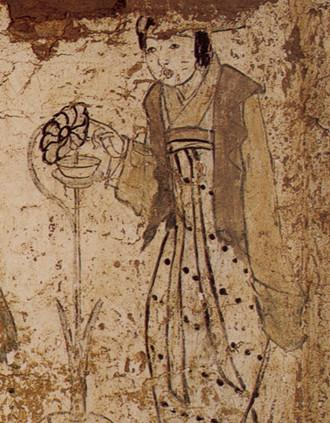
\includegraphics[width=\textwidth]{images/heyedeng.jpg}
     \end{subfigure}
     \hfill
     \begin{subfigure}[H]{0.45\textwidth}
         \centering
         \caption*{87版电视剧中的荷叶灯}
         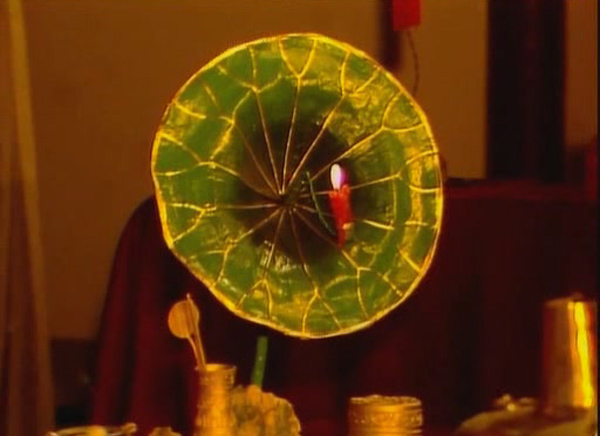
\includegraphics[width=\textwidth]{images/87heyedeng.jpg}
     \end{subfigure}  
\end{figure}
}:古代灯罩的基本作用是防风雨、吸纳烟灰、聚光,可以转动与开合的灯罩能够调整灯照角度、亮度。
荷叶灯是用荷叶形状的挡光板做灯罩的灯具。
荷叶呈聚拢状,有聚光的作用。
为了增强反光能力,在荷叶表面覆盖具有玻璃光泽的珐琅涂层。
可以通过调整荷叶的位置和角度,调节光的角度。
}窗格门户一齐摘下,
\zhu{窗格:亦称“窗隔”、“窗槅”。窗上的格子,古时在上面糊纸或纱以挡风,亦指窗扇。}
全挂彩穗各种宫灯。
廊檐内外及两边游廊罩棚,将各色羊角、玻璃、戳纱、料丝、\zhu{羊角、玻璃、戳纱、料丝都是灯罩的材料。
羊角:即羊角灯,又叫明角灯,用透明角质材料为罩的灯,半透明,能防风雨。
戳纱:一种有明显竖向纹理的纱。
料丝:以玛瑙、紫石英等熔化后抽丝而成的一种透光材料。
}或绣、或画、或堆、或抠、或绢、或纸诸灯挂满。
\par
廊上几席,便是贾珍、贾琏、贾环、贾琮、贾蓉、贾芹、贾芸、贾菱、贾菖等。
贾母也曾差人去请众族中男女,奈他们或有年迈懒于热闹的;或有家内没有人不便来的;或有疾病淹缠,欲来竟不能来的;或有一等妒富愧贫不来的;甚至于有一等憎畏凤姐之为人而赌气不来的;或有羞手羞脚,不惯见人,不敢来的:因此族众虽多,女客来者只不过贾菌之母娄氏带了贾菌来了,男子只有贾芹、贾芸、贾菖、贾菱四个现是在凤姐麾下办事的来了。
当下人虽不全,在家庭间小宴中,数来也算是热闹的了。
\par
当下又有林之孝之妻带了六个媳妇,抬了三张炕桌,每一张上搭着一条红毡,毡上放着选净一般大新出局的铜钱,用大红彩绳串着,每二人搭一张,共三张。
林之孝家的指示将那两张摆至薛姨妈李婶的席下,将一张送至贾母榻下来。
贾母便说:“放在当地罢。
”这媳妇们都素知规矩的,放下桌子,一并将钱都打开,将彩绳抽去,散堆在桌上。
\par
正唱《西楼·楼会》这出将终,\zhu{《西楼记》:明末清初袁于令所作。该剧描写于叔夜和妓女穆素徽悲欢离合的故事。
第八出《病晤》的演出本叫《楼会》,俗称《西楼会》,写于叔夜专程来访,穆素徽抱病出见,二人定情事。
下回的楚江晴即《楼会》中的一支曲子。
}于叔夜因赌气去了,那文豹便发科诨道:\zhu{
诨:音“混”,指古代戏曲中逗笑的台词。
科诨:插科打诨的简称,指穿插在戏曲中令人发笑的滑稽动作和对话。
}“你赌气去了,恰好今日正月十五,荣国府中老祖宗家宴,待我骑了这马,赶进去讨些果子吃是要紧的。
”说毕,引的贾母等都笑了。
薛姨妈等都说:“好个鬼头孩子,可怜见的。
”凤姐便说:“这孩子才九岁了。
”贾母笑说:“难为他说的巧。
”便说了一个“赏”字。
早有三个媳妇已经手下预备下小簸箩,听见一个“赏”字,走上去向桌上的散钱堆内,每人便撮了一簸箩,走出来向戏台说:“老祖宗、姨太太、亲家太太赏文豹买果子吃的!”说着,向台上便一撒,只听豁啷啷满台的钱响。
\par
贾珍贾琏已命小厮们抬了大簸箩的钱来,暗暗的预备在那里。
听见贾母一赏,要知端的——\par
\qi{总评:叙元宵一宴,却不叙酒何以清,菜何以馨,客何以盛,令何以行。
先于香茗古玩上渲染,几榻坐次上铺陈,隐隐为下回张本,有无限含蓄,超迈獭祭者百倍。
\zhu{獭祭:音“塔寄”,即“獭祭鱼”,谓獭常捕鱼陈列水边,如同陈列供品祭祀。
实际上因獭食鱼往往只吃一两口就抛掉,捕鱼能力又强,所以每食必抛掉许多吃剩的鱼。
比喻罗列典故或堆砌成文。
}\hang
前半整饬,\zhu{整饬:音“整赤”,整齐有序,端庄严谨。
}后半疏落,浓淡相间。
祭宗祠在宁府,开夜宴在荣府,分叙不犯手,\zhu{犯:这里是重复之意。
}是作者胸有成竹处。
}
\dai{105}{乌进孝向贾府交租}
\dai{106}{元宵看戏贾母放赏,用簸箩撒钱}
\sun{p53-1}{宁国府除夕祭宗祠}{贾氏宗祠正堂上,影前锦幔高挂,彩屏张护,香烛辉煌。
上面正居中悬着宁荣二祖遗像,皆是披蟒腰玉。
槛外方是贾敬贾赦,槛内是各女眷,众家人小厮皆在仪门之外。
每一道菜按次传至贾敬手中,又依次直传于贾母。
}
\sun{p53-2}{荣国府元宵开夜宴}{贾母在大花厅上命摆几席酒,定一班小戏,满挂各色佳灯,带领荣宁二府各子侄孙男孙媳等家宴。
}